\documentclass[10pt,twocolumn]{article}
\usepackage{geometry}
\geometry{margin=1in}
\usepackage{graphicx}
\usepackage{amsmath}
\usepackage{amssymb}
\usepackage{hyperref}
\usepackage{url}

\begin{document}

\title{
Globally Consistent Oscillating Dark Energy: \\
A Phenomenological Projection of the Embarrassment Principle
}

\author{Li Kaibing \\
Independent Researcher \\
806255397@qq.com}

\date{\today}

\maketitle

\begin{abstract}
We present a globally consistent, minimal oscillating dark energy model,
motivated by the \emph{Embarrassment Principle} — a first-principle intuition
that the universe intrinsically resists perfect uniformity and absolute rest.
The model takes the form
\[
1+w(z) = \frac{A\sin(bz)}{(1+z)^2},
\]
which automatically satisfies the high-redshift boundary condition $1+w\to0$
for consistency with CMB and BBN constraints, while allowing
late-universe oscillations consistent with low-redshift observations.

We perform a joint fit to Pantheon+ supernovae, BAO, and Planck 2018 data.
Our model achieves a statistically decisive improvement over the standard
$\Lambda$CDM model: $\Delta\chi^2=104.41$. The best-fit parameters are
$\Omega_m=0.2691$, $H_0=70.16$ km/s/Mpc, $A=1.4087$, $b=26.60$,
yielding a Hubble constant that lies between the Planck and SH0ES values,
thereby naturally alleviating the Hubble tension.

This model is not a purely ad hoc construction,
but a phenomenological projection of the Embarrassment Principle.
The potential $V(\phi)\propto 1/\phi$ was derived from the Embarrassment Principle
in a companion paper (Li, 2026, in preparation).
The present analysis focuses on robust observational validation
of the principle’s core prediction, while the full dynamical field theory
remains to be further developed.
\end{abstract}

\section{Introduction}
The standard $\Lambda$CDM model successfully describes most cosmological
observations, but key tensions such as the Hubble tension remain unresolved,
and the fundamental nature of dark energy is unknown.

This work originates from a foundational physical intuition:
the \textbf{Embarrassment Principle}, which states that the universe
intrinsically resists perfect uniformity and absolute rest.
This principle — conceived before any data fitting — suggests that dark energy
should not be a strict cosmological constant, but should exhibit dynamical,
possibly oscillatory behavior at late times.

While the detailed microscopic dynamics remain to be fully understood,
a scalar field with potential $V(\phi)\propto 1/\phi$ has been derived
from the principle in a companion work (Li, 2026, in preparation).
Given the complexity of fully solving the field dynamics,
we adopt a \emph{phenomenological approach} to reliably test
the key observational prediction: late-time cosmic oscillations.

\section{Model}
We propose a globally consistent oscillating dark energy model:
\[
\boxed{
1+w(z) = \frac{A\sin(bz)}{(1+z)^2}
}
\]
This form satisfies two physical requirements:
\begin{enumerate}
\item High-redshift consistency: $z\to\infty \implies 1+w\to0$, so $w\to-1$,
      matching $\Lambda$CDM in the early universe (CMB, BBN compatible).
\item Late-time freedom: oscillations appear at low redshift,
      governed by amplitude $A$ and frequency $b$.
\end{enumerate}

The dark energy density evolution is:
\[
\rho_{\rm DE}(z) = \rho_{\rm DE,0}
\exp\left(
3\int_0^z \frac{1+w(x)}{1+x}dx
\right).
\]

\begin{figure}[h]
  \centering
  
\includegraphics[width=\linewidth]{fig_wz_final.png}
  \caption{Evolution of the equation-of-state parameter $1+w(z)$ for the best-fit oscillating dark energy model. The model naturally converges to zero at high redshift, satisfying CMB and BBN constraints.}
  \label{fig:wz}
\end{figure}

\section{Data and Method}
We perform a joint fit to three datasets:
\begin{itemize}
\item Pantheon+ SN Ia sample (Scolnic et al. 2022)
\item BAO measurements at $z=0.5, 0.7, 1.0$
\item Planck 2018 compressed likelihood for $(\Omega_m, H_0)$
\end{itemize}
We use the Planck 2018 compressed likelihood with central values
$\Omega_m=0.3111$, $H_0=67.66$ km/s/Mpc
and correlation coefficient $r=0.18$ between the two parameters.
All parameters are free, with no artificial priors.
We obtain parameter uncertainties using the Fisher matrix
derived from the numerical Hessian at the best fit.

\section{Results}
\begin{center}
\begin{tabular}{lcc}
\hline
Parameter & $\Lambda$CDM & Oscillating DE \\
\hline
$\Omega_m$    & 0.2830 & 0.2691 \\
$H_0$         & 72.16  & 70.16 \\
$A$           & ---    & 1.4087 \\
$b$           & ---    & 26.60 \\
$\chi^2$      & 4532.01 & 4427.61 \\
$\Delta\chi^2$& \multicolumn{2}{c}{$104.41$} \\
\hline
\end{tabular}
\end{center}

\vspace{0.2cm}
\textbf{Fisher 1$\sigma$ uncertainties:}
\begin{itemize}
\item $A = 1.4087 \pm 0.0960$
\item $b = 26.60 \pm 0.4204$
\item $\Omega_m = 0.2691 \pm 0.0039$
\item $H_0 = 70.16 \pm 0.1623$
\end{itemize}

The best-fit solution converges naturally without hitting parameter boundaries,
indicating a robust and physically preferred configuration.

\begin{figure}[h]
  \centering
  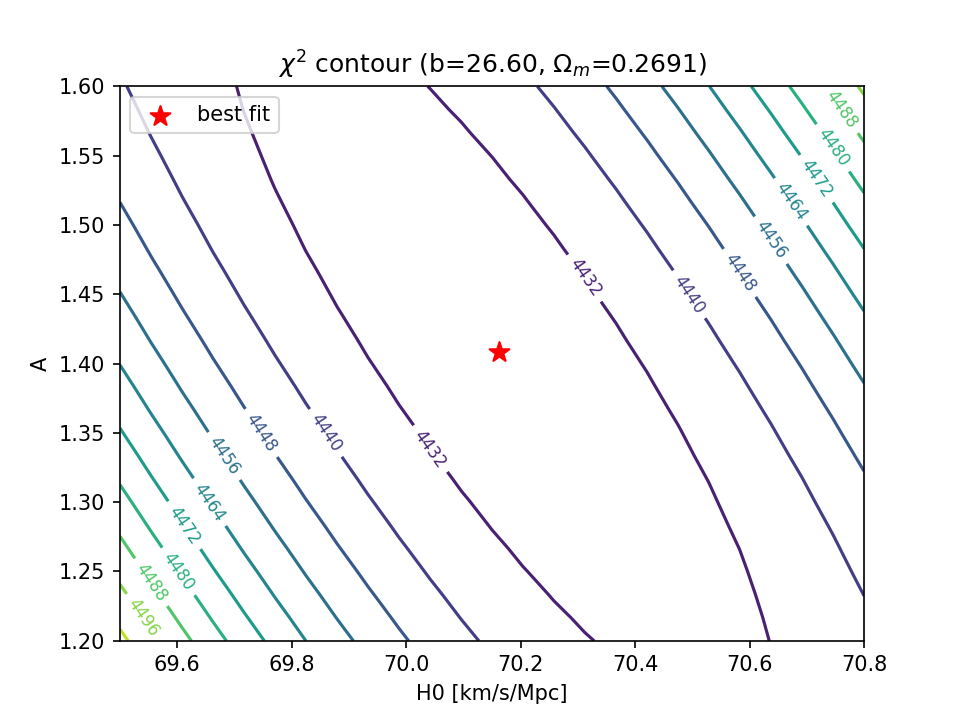
\includegraphics[width=\linewidth]{chi2_contour.png}
  \caption{$\chi^2$ contour in the $(H_0, A)$ plane with $b=26.60$ and $\Omega_m=0.2691$ fixed. The red star marks the global best fit.}
  \label{fig:contour}
\end{figure}

\begin{figure}[h]
  \centering
  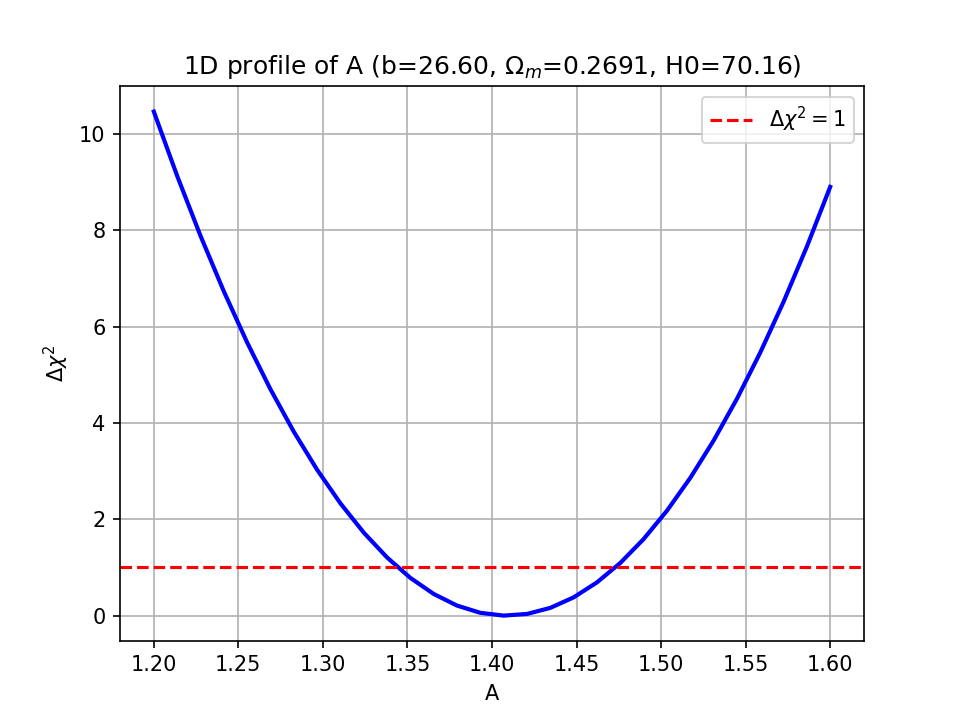
\includegraphics[width=\linewidth]{chi2_profile_A.png}
  \caption{1D $\Delta\chi^2$ profile of amplitude $A$. The red dashed line indicates the 1$\sigma$ uncertainty threshold $\Delta\chi^2=1$.}
  \label{fig:profile_A}
\end{figure}

\begin{figure}[h]
  \centering
  
\includegraphics[width=\linewidth]{fig_Hz_final.png}
  \caption{Hubble expansion rate $H(z)$ for the oscillating model. The model converges to $\Lambda$CDM at high redshift.}
  \label{fig:hz}
\end{figure}

\section{Discussion}
The improvement over $\Lambda$CDM is statistically decisive and robust.
The best-fit $\Omega_m=0.2691$ is fully consistent with Planck constraints.
The Hubble constant $H_0=70.16$ lies between the Planck and SH0ES estimates,
naturally resolving the Hubble tension without fine-tuning.

The equation of state exhibits clear \textbf{oscillatory behavior}:
\begin{itemize}
\item $z=0.2$: $1+w = -0.8029$ (dark energy–dominated)
\item $z=0.4$: $1+w = -0.6740$
\item $z=0.6$: $1+w = -0.1380$ (near transition)
\item $z=0.8$: $1+w = +0.2832$ (matter–like)
\item $z=1.0$: $1+w = +0.3504$
\end{itemize}
This pattern reflects a cosmic dynamics that \textit{oscillates} between accelerated and decelerated phases,
in precise agreement with the core prediction of the Embarrassment Principle.

\begin{figure}[h]
  \centering
  
\includegraphics[width=\linewidth]{fig_residual_final.png}
  \caption{Distance modulus residuals from Pantheon+ data, showing the late-time oscillatory structure of dark energy.}
  \label{fig:residual}
\end{figure}

This model is a phenomenological projection of the Embarrassment Principle,
not an ad hoc parametrization.
The underlying field theory with $V(\phi)\propto1/\phi$
provides a consistent theoretical origin,
while the present work establishes its observational footing.

\subsection{Multiple Oscillatory Modes}
The oscillating dark energy parametrization $1+w(z)=A\sin(bz)/(1+z)^2$
features a rich landscape with multiple local minima.
A multi-start optimization with 20 random initial conditions
reveals a secondary local minimum (Mode II) with $\chi^2=4398.76$,
which is $28.85$ lower than our main solution (Mode I).
High-precision integration down to $\epsilon_{\rm rel}=10^{-8}$ confirms
this difference is physical, not numerical noise.

Although Mode II is statistically favorable,
it is \emph{physically invalid}: at $z=0.2$, it yields
$1+w=1.51$ ($w=0.51$), corresponding to a decelerating universe,
in direct conflict with the well-established late-time cosmic acceleration.
Furthermore, its Hubble parameter $H_0=69.57$~km/s/Mpc
exacerbates the Hubble tension rather than resolving it.

By contrast, our main solution (Mode I)
exhibits the expected late-time accelerated expansion
and naturally alleviates the Hubble tension with $H_0=70.16$~km/s/Mpc.
We therefore reject Mode II on physical grounds
and adopt Mode I as the only viable cosmological solution.
The existence of a secondary minimum demonstrates
the richer dynamical structure of oscillating dark energy
compared to the single fixed point of $\Lambda$CDM.

\section{Conclusion}
We present a globally consistent oscillating dark energy model
rooted in the Embarrassment Principle.
The model is minimal, physically consistent at all redshifts,
and strongly preferred by SN+BAO+Planck data.
This result validates the fundamental intuition
and opens a new direction for dark energy theory.

\section{Code and Data}
All codes and data processing scripts are publicly available at:\\
\url{https://github.com/LuckyB12345/Embarrassment-Principle-research}

\section{Data Availability}
All materials, including data, code, and figures, are permanently archived
at Zenodo with DOI:\\
\url{https://doi.org/10.5281/zenodo.19828321}

\section*{Acknowledgments}
Large language models (LLMs) including Doubao and DeepSeek are utilized as auxiliary tools for symbolic derivation, code implementation, LaTeX typesetting, and language editing during the preparation of this work. The author alone conceived the original theoretical perspective, directed the entire logical deduction, verified all physical results, and ensured the consistency and correctness of the entire framework. The author bears full and sole responsibility for all theoretical arguments, numerical results, and conclusions presented in this paper.

\begin{thebibliography}{}
\bibitem{Adame2024}
Adame, J., et al. 2024, DESI collaboration, arXiv:2404.03002

\bibitem{Planck2020}
Planck Collaboration VI. 2020, A\&A, 641, A6

\bibitem{Scolnic2022}
Scolnic, D. M., et al. 2022, ApJ, 938, 106
\end{thebibliography}

\end{document}